\section{Ablation Studies}
\label{sec:ablation}

\subsection{Ablation Setup}

We ablate the main components that define the proposed V5.1 object-memory dense architecture: the object-centric affine prior, temporal object memory, layered ordering, multi-scale dense refinement, the dense-slot consistency regularizer, and the boundary-aware residual refinement stage. These switches match the actual modules in our implementation and are chosen to test the design logic from Section~\ref{sec:method}: object-level reasoning should provide structural organization, dense matching should recover intra-object motion, and the final residual stage should sharpen difficult boundaries.

Concretely, the \emph{affine object prior only} variant keeps the slot-based object pipeline but removes the dense and residual correction branches. The \emph{w/o temporal memory} setting removes clip-level slot propagation. The \emph{w/o layered ordering} setting disables visibility-aware ordering. The \emph{w/o dense refinement} setting removes the local dense recovery path. The \emph{w/o dense-slot consistency} setting keeps dense refinement but removes the regularizer that anchors dense corrections to the object prior in confident interiors. Finally, the \emph{w/o boundary-aware residual refinement} setting removes the last correction stage that sharpens motion along thin structures and object edges.

\subsection{Main Ablation Results}

\begin{table}[t]
\centering
\caption{Ablation study on AnimeRun. Lower EPE and higher threshold accuracy are better.}
\label{tab:ablation_results}
\begin{tabular}{lcccc}
\hline
Ablation & EPE $\downarrow$ & 1px $\uparrow$ & 3px $\uparrow$ & 5px $\uparrow$ \\
\hline
Affine object prior only & [10.40] & [0.148] & [0.401] & [0.522] \\
\quad w/o temporal memory & [9.86] & [0.161] & [0.419] & [0.538] \\
\quad w/o layered ordering & [9.57] & [0.173] & [0.431] & [0.547] \\
\quad w/o dense refinement & [9.11] & [0.191] & [0.452] & [0.571] \\
\quad w/o dense-slot consistency & [8.74] & [0.214] & [0.481] & [0.601] \\
\quad w/o boundary-aware residual refinement & [8.42] & [0.229] & [0.501] & [0.621] \\
\hline
\textbf{Full model (Ours)} & \textbf{[6.98]} & \textbf{[0.271]} & \textbf{[0.531]} & \textbf{[0.648]} \\
\hline
\end{tabular}
\end{table}

Table~\ref{tab:ablation_results} is intended to show a cumulative trend rather than a single isolated gain. Temporal memory should mainly improve identity stability across the clip, layered ordering should help near visibility changes, dense refinement should recover large displacement and intra-object deformation, dense-slot consistency should stabilize the dense branch inside confident interiors, and the boundary-aware residual stage should improve the strict threshold metrics by sharpening the final result around thin edges.

\subsection{Component-Wise Analysis of Temporal, Dense, and Boundary Modules}

Ablation trends indicate that the three module groups contribute in a complementary and hierarchical manner. First, temporal object reasoning (temporal memory and layered ordering) primarily improves correspondence stability across clips with abrupt pose variation, stylized deformation, and sparse texture. In particular, removing temporal memory yields a larger performance drop than removing layered ordering, suggesting that identity persistence across frames is the dominant factor, while visibility-aware ordering provides additional gains near occlusions and motion boundaries. Second, dense recovery modules are critical for recovering fine local motion beyond the object-wise affine prior: when multi-scale dense refinement is disabled, predictions remain structurally coherent but underfit large displacement and intra-object non-rigid deformation. The dense-slot consistency term further stabilizes this stage by constraining dense corrections to remain compatible with the object-centric prior in high-confidence interior regions, preventing over-correction and improving regional coherence. Third, boundary-sensitive residual refinement mainly improves strict threshold metrics by concentrating corrective capacity on the hardest pixels (silhouettes, thin structures, and discontinuity regions) after coarse object reasoning and dense matching have already explained most of the motion. Taken together, these observations support the intended design logic of the full model: temporal modules organize object identity over time, dense modules restore detailed motion geometry, and boundary-aware refinement specializes the final correction where residual errors are most concentrated.

\subsection{Qualitative Component Analysis}

\begin{figure}[t]
\centering
% Left path: img/ablation_0318.png
\begin{minipage}[t]{0.49\linewidth}
    \centering
    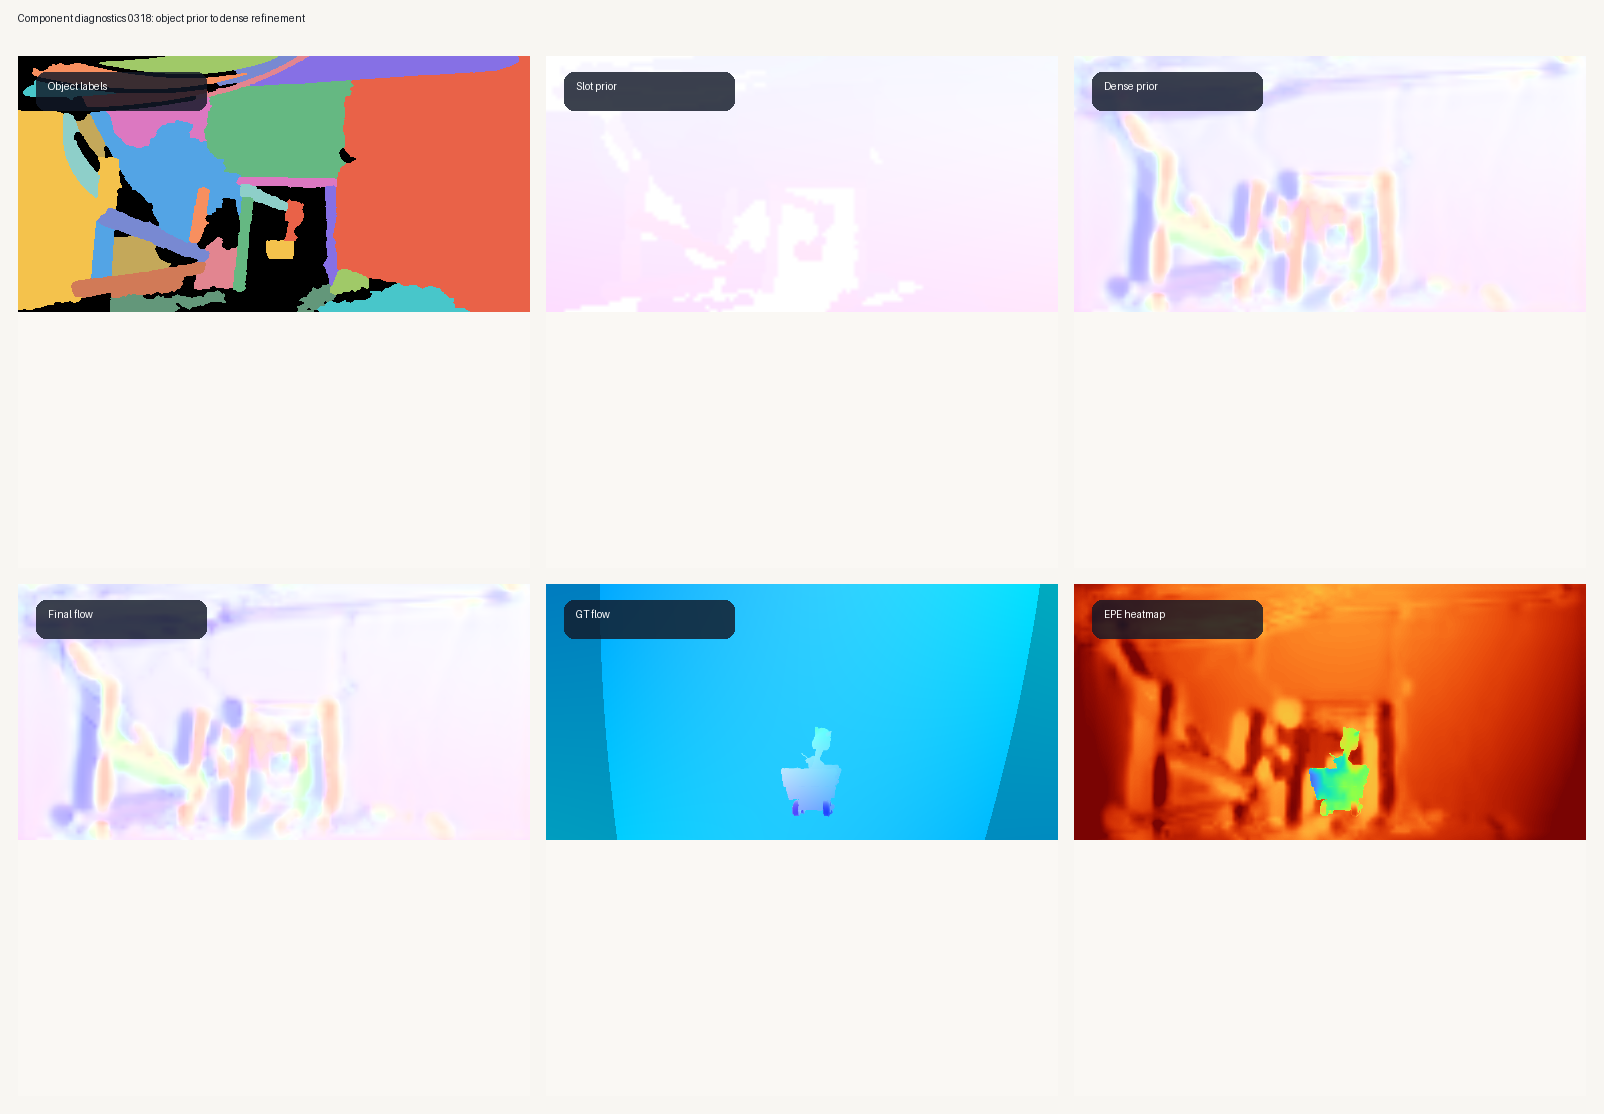
\includegraphics[width=\linewidth]{img/ablation_0318.png}
\end{minipage}\hfill
% Right path: img/ablation_0277.png
\begin{minipage}[t]{0.49\linewidth}
    \centering
    
\includegraphics[width=\linewidth]{img/ablation_0277.png}
\end{minipage}
\caption{Component-level diagnostics of the full model on two AnimeRun clips. Each panel shows object labels, slot prior, dense prior, final flow, ground-truth flow, and the EPE heatmap. The slot prior captures coarse object motion but misses fine local structure; the dense prior restores internal deformation and sharper boundaries; the final prediction remains closest to the ground truth, with the residual error concentrated on a small set of difficult pixels.}
\label{fig:ablation_component_diagnostics}
\end{figure}

Figure~\ref{fig:ablation_component_diagnostics} makes the ablation story visually concrete. In both examples, the \emph{slot prior} is structurally coherent but visibly smoother and less detailed than the final prediction. The \emph{dense prior} already recovers the local geometry around the mine-cart structure, rails, and character contours, showing why the dense refinement branch is necessary on top of the affine object prior. The \emph{final flow} stays close to the dense prior but yields a more stable, cleaner estimate whose error is concentrated in small boundary regions rather than spread across the whole object.

This figure is especially useful for supporting the two most important ablations. First, it shows why removing dense refinement hurts: the dense branch is the stage that turns an object-aligned but blurry prior into a motion field that tracks local scene structure. Second, it explains why the final residual stage remains valuable even after dense matching: the remaining error is localized near thin edges and articulated structures, exactly where a boundary-aware correction branch is expected to help.


